\begin{frame}[fragile,label=homesModelExer]{exercise: holes in the model?}
\begin{tikzpicture}
\node (left) {
\begin{lstlisting}[language=C++,style=smaller]
void example(int a) {
    int *p;
    int *q;
    q = malloc(...);
    p = malloc(...);
    // (A)
    if (a > 0) {
        // (A1)
        p = q;
    }
    // (B)
    free(p);
    // (C)
    ...
}
\end{lstlisting}
};
\node[anchor=north west,align=left,draw,very thick] at (left.north east) {
exercise: what should state of pointer q be at C? \\
A. allocated \hspace{.5cm} B. freed \\
C. allocated if+only if reached via path with A1\\
D. freed if+only if reached via path with A1 \\
E. something else?
};
\end{tikzpicture}
\end{frame}

\begin{frame}{clang-analyzer output}
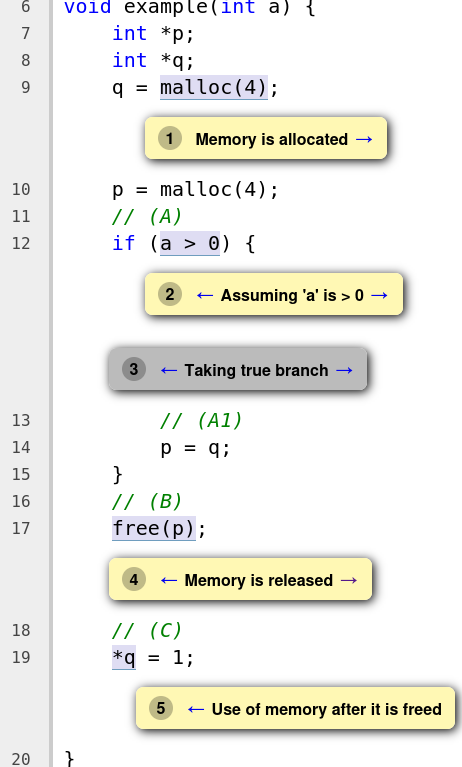
\includegraphics[height=0.9\textheight]{../static/clang-analyze-example4}
\end{frame}
